\section{Einleitung} \label{sec:einleitung}
Diese Arbeit beschäftigt sich mit der Thematik \textit{\textbf{\glqq Künstliche Intelligenz\grqq{}}}. Künstliche Intelligenzen sind Forschungsgegenstand der Neuroinformatik. (\vgl \cite[3]{Schaeffer2021}). Speziell der Zweig der \textbf{künstlichen neuronalen Netze} (engl.\xspace Artificial Neural Network ANN) spielt immer mehr eine große Rolle für reale Anwendungsfälle. Prominente Beispiele sind unter anderem das autonome Fahren und die Worterkennung bei Sprachassistenten. (\vgl \cite[15]{Styczynski2017}). \\
Künstliche neuronale Netzwerke (im Folgenden abgekürzt mit KNN) sind Netze aus künstlichen Neuronen. Dabei handelt es sich um ein Modell nach dem biologischen Vorbild einer Nervenzelle. (\vgl \cite[136,137]{Styczynski2017}). Eine spezielle Form der neuronalen Netze sind die \textbf{Convolutional Neural Networks} (im Folgenden abgekürzt mit CNN). Der Name resultiert aus der Anwendung der Faltung  bei der Nutzung dieses Netzwerktyps. Es handelt sich auch hier um ein von biologischen Prozessen inspiriertes Konzept im Bereich des \textbf{maschinellen Lernens}. (\vgl \cite[50]{Prakash2021}). \\
In dieser Arbeit soll zunächst theoretisch das Konzept und die Funktionsweise der CNN beleuchtet werden. Dabei wird vor allem auch auf \textbf{AlexNet} als beispielhaftes CNN eingegangen, da dieses im späteren Verlauf Anwendung findet. Darauf aufbauend wird im Anschluss das \textbf{Transfer-Learning} erklärt. Auch dieses soll verwendet werden.

\begin{wrapfigure}{r}{0.5\textwidth}
    \centering
   \fbox{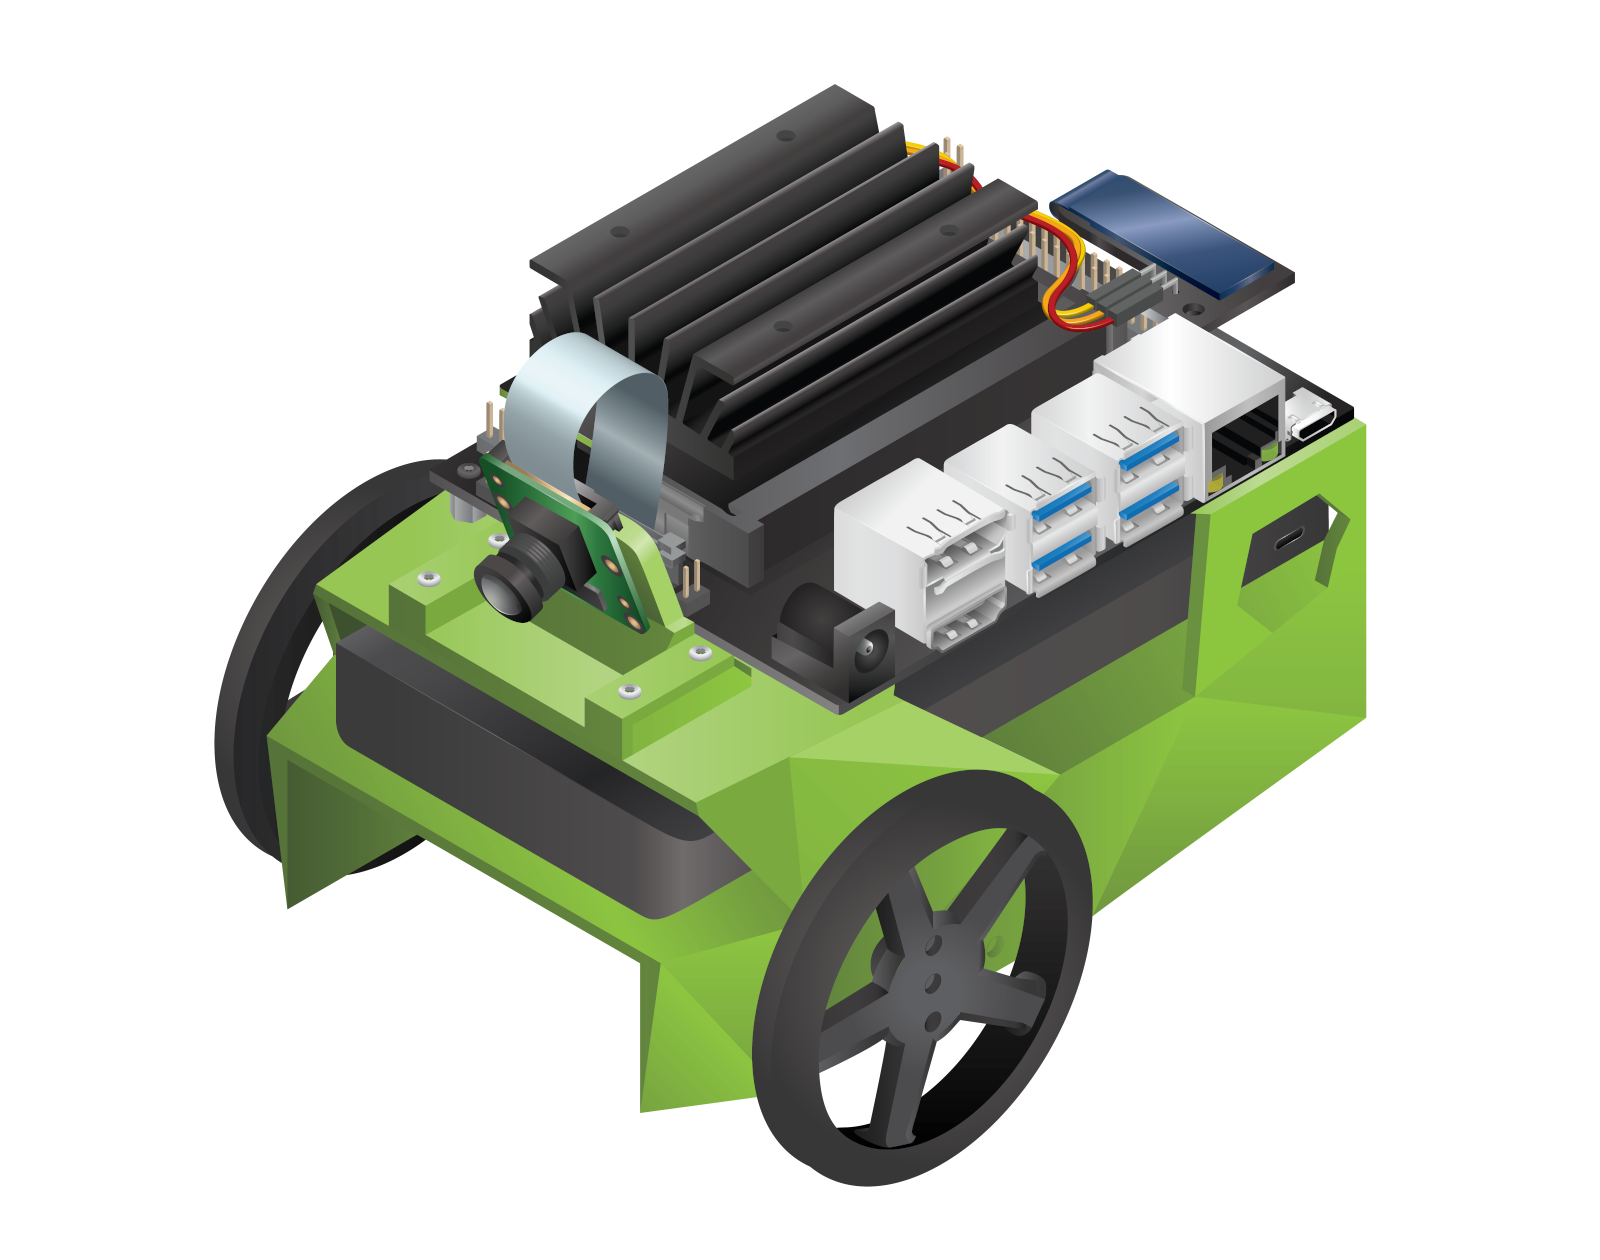
\includegraphics[width=0.48\textwidth]{Bilder/jetbot-illustration.png}}
   \caption[Illustration Jetbot Roboterfahrzeug]{Illustration des Jetbot Roboterfahrzeugs}
   \label{fig:Bild1.1}
\end{wrapfigure}

Abschließend wird die Arbeit mit der Anwendung der behandelten Konzepte an einem praktischen Versuch getestet. Hierzu sollen in Echtzeit Bilddaten von einer Kamera auf einem kleinen Roboterfahrzeug mittels CNN und Transfer-Learning ausgewertet werden, so dass das Gefährt sich kollisionfrei im Raum fortbewegen kann. Sämtliche Berechnungen als auch die Steuerung des Roboters werden auf einem \textbf{Jetson Nano} Mikrocontroller des Unternehmens Nvidia durchgeführt. Dieses ist bekannt für die Produktion von (Hochleistungs-) Grafikkarten (kurz GPU - Graphical Processing Unit). Der Jetson Controller ist ebenfalls mit einer GPU ausgestattet, die es ermöglicht rechenintensive Operationen, wie \zB die Berechnung von neuronalen Netzen durchzuführen. \\
Die \autoref{fig:Bild1.1} zeigt den Jetson Nano Controller auf dem Roboterfahrzeug \textit{\glqq Jetbot\grqq{}} inklusive einer kleinen Weitwinkelkamera.